\section{Dog alarm}\label{sec:dog-alarm}
Jednou z klíčových komponent systému Coopmaster je služba pro ochranu slepic před potenciálním nebezpečím ve výběhu, nesoucí název Dog Alarm.
Za využití modelu Yolo11 služba detekuje vetřelce (psa) na fotkách z kamery ve výběhu a informuje pomocí MQTT protokolu chovatele do systému Home Assistant.

\subsection*{Obecný princip}
Jako zdroj dat je použit kamerový systém ve výběhu, který je reprezentován službou Camera Driver.
Z této služby pak Dog Alarm stahuje pomocí GET požadavků fotografie z kamery ve výběhu.\newline

Pro detekci predátorů je využito modelu Yolo11.
Model je velmi kvalitně vyučený a společnost Ultralytics~\cite{ultralytics} k němu nabízí rozsáhlou dokumentaci, což je také jeden z hlavních důvodů mojí volby.
Před nasazením jsem model ještě doučit o další fotografie psa pořízené z venkovní kamery, podobně jako je to v sekci~\ref{sec:detekce-objektu-pomoci-strojoveho-uceni}, aby se model více přizpůsobil podmínkám vstupních fotografií.\newline

Jakmile model identifikuje přítomnost psa nebo jiného predátora, služba Dog Alarm okamžitě vygeneruje výstrahu.
Tato výstraha je odeslána pomocí protokolu MQTT do systému Home Assistant.
Spolu se zprávou je připojen specifický záběr, na kterém byl predátor detekován, aby mohl chovatel zhodnotit situaci sám.\newline

Kromě výstražných zpráv, Dog Alarm pravidelně zasílá aktuální záběry z kamery do Home Assistanta, čímž umožňuje uživatelům mít průběžný přehled o situaci ve výběhu.\newline

\subsection*{Popis algoritmu}
Po startu služby se inicializuje REST API vytvořené pomocí Flask frameworku.
Toto API poskytuje endpoint pro volání služby Health Checker s dotazem na stav služby.
Následně je spuštěn scheduler, který má za úkol jednou za minutu spustit job s názvem check\_dog.
Jako poslední je spuštěno poskytování REST API na portu 9008.\newline

\subsection*{Popis algoritmu pro job check\_dog}
Tento job detekuje vetřelce a stará se o report informací.
Prvním krokem jobu je stažení aktuálního obrázku z kamery ve výběhu.
Další následuje načtení příslušného Yolo modelu dle konfigurace.
Následně je provedena detekce objektů v obraze (ukázka výsledku je na obrázku~\ref{fig:dog_detected}), o čemž se dále rozepisuji v sekci~\ref{sec:detekce-objektu-pomoci-strojoveho-uceni}.
Výsledný seznam detekovaných objektů se analyzuje a zjistí se, zda obsahuje kategorii pes.
Před koncem jobu se stav, zda byl detekován pes publiku na MQTT topic coopmaster/dog/detected a aktuální obrázek na topic coopmaster/dog/image/actual.
Tyto MQTT topics odebírá systém Home Assistant a dále s nimi pracuje což je popsáno v sekci~\ref{sec:tvorba-gui-rozhrani}.

\begin{figure}[H]
    \centering
    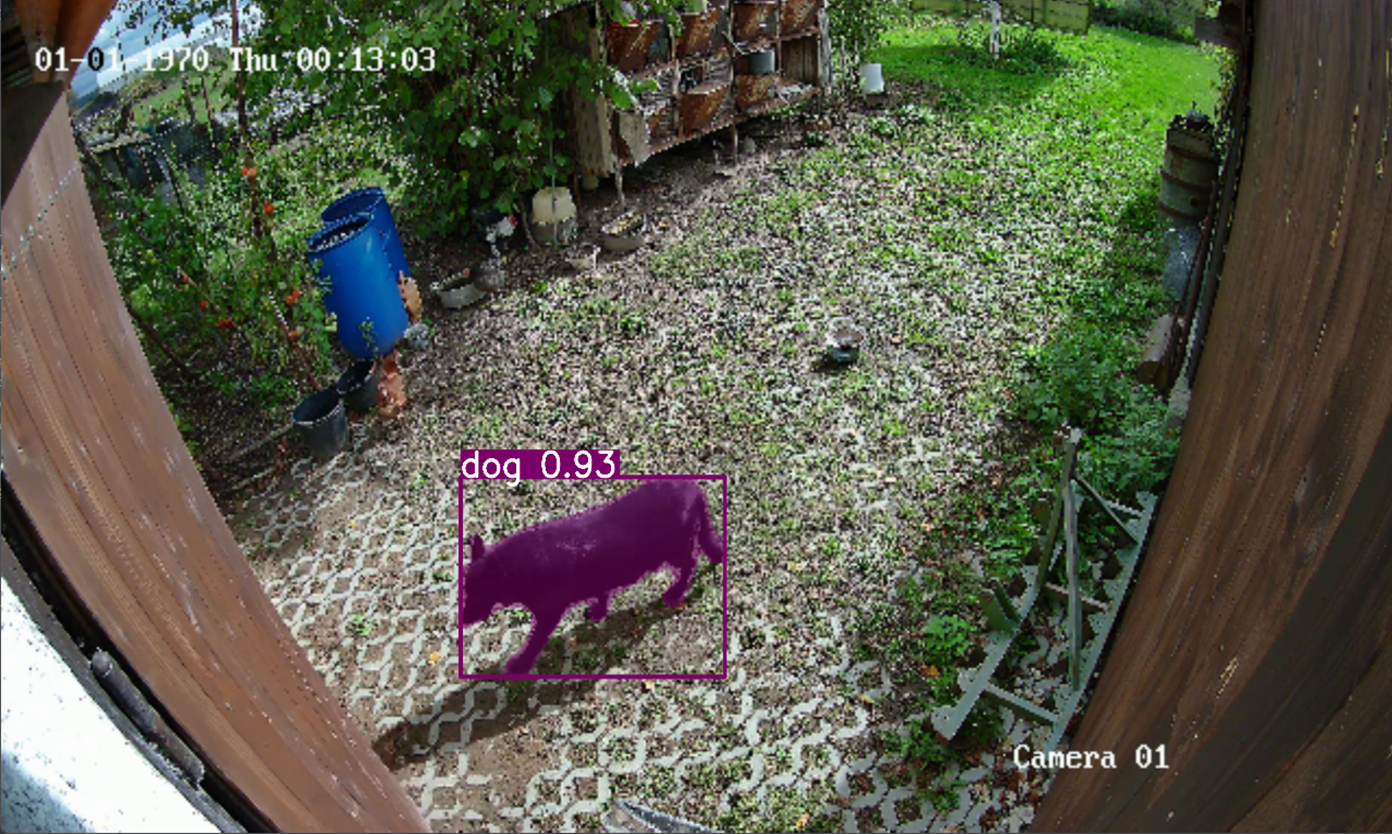
\includegraphics[width=0.8\textwidth]{img/dog_detected}
    \caption{Pes detekován ve výběhu}
    \label{fig:dog_detected}
\end{figure}



%\subsection*{Výhody a přínosy}
%
%Implementace Dog Alarm v systému Coopmaster nabízí několik klíčových výhod:
%\begin{itemize}
%    \item \textbf{Automatizovaný dohled:} Automatická detekce predátorů výrazně zvyšuje bezpečnost slepic tím, že minimalizuje závislost na lidském dohledu.
%    \item \textbf{Rychlá reakce:} Díky okamžitému odesílání upozornění může být rychle aktivována ochranná opatření.
%    \item \textbf{Dokumentace incidentů:} Uložení snímků predátorů poskytuje důležitou dokumentaci pro další analýzu a případné právní kroky.
%\end{itemize}
%Služba Dog alarm má detekovat nebezpečí ve výběhu a poslat tuto zprávu do Home Assistanta.\newline
%Aktuální záběry jsou pomocí GET requestů stahovány z konkrétní instance služby Camera driver, která je přiřazena ke kameře ve výběhu.
%Analýza probíhá v určitých intervalech za pomocí umělé inteligence, kde je konkrétně použita metoda detekce objektů.
%Jakmile jako výsledek klasifikace vyjde jednoznačně, že v záběru byl spatřen pes nebo jiný predátor, je zpráva poslána pomocí MQTT do Home Assistanta společně s konkrétním záběrem, na němž byl predátor detekován.
%Tato služba zároveň přes MQTT posílá do Home Assistanta aktuální záběr z kamery.
